

The application of the zeroth order equation have been dealt in numerous article in the fields therefore it won't be more detailed in this study. 
\tb{interesting to notice that it has the same shape regardless of the nature of the partcle EXCEPT WHEN CHANGES OF MASS APPEAR}

Regarding, the first order moments equations may seem useless. 
That is why we would like to revisit the ideas and to show how they are in fact already  used in numerous cases. 

\subsubsection*{Solid axis symmetric particles}

Let's start by the second moment of mass averaged equation. 
Even through if it is a second order equation we quickly recognize that it is of a major important in the case of elongated particle suspension for example. 
Indeed, Let the vector $\textbf{p}$ be the orientation of the particle along its axe.
Then the second moment of mass can be written as $\mathcal{M}_\alpha =  \textbf{pp} (M_\alpha^{||} - M_\alpha^\bot) +  \textbf{I} M_\alpha^\bot$, with $M_{\bot}$ and $M_{||}$ coefficient equivalent to the principal direction of the mass distribution.
It is then possible to demonstrate that the second moment of mass correspond to the transport equation of the orientation tensor $\textbf{A}=\avg{\delta_\alpha\textbf{pp}} = \pnavg{\textbf{pp}}$. 
In this situation, $\pnnavg{\mathcal{M}_\alpha} =  \textbf{A} (M_\alpha^{||} - M_\alpha^\bot) +  \textbf{I} M_\alpha^\bot$. 
Then, assuming torque free rigid particle in to Stokes flow regime, we obtain by averaging  \ref{eq:dt_M_alpha} the following equation :
\begin{equation}
    \pddt \textbf{A}
    + \nablab \cdot (
        \pnnavg{\textbf{u}_\alpha}\textbf{A}
    )
    = 
    \mathbf{\Omega} \cdot \textbf{A}
    - \textbf{A} \cdot \mathbf{\Omega} 
    + \beta\left[
        \textbf{E} \cdot \textbf{A}
        -\textbf{A} \cdot \textbf{E} 
        - \textbf{E} : \mathbb{A}
    \right]
    - \nablab \cdot \mathbf{\Sigma}
    \label{eq:hybrid_avg_dt_pp}
\end{equation}
where $\textbf{D}$ and $\mathbf{\Omega}$ are the symmetric and antisymmetric parts of the bulk velocity gradient, $\nablab\avg{\textbf{u}}$, the fourth-order $\mathbb{A}$ is defined such as $\mathbb{A} = \pnavg{\textbf{pppp}}$ and $\mathbf{\Sigma} = \pnavg{\textbf{u}'_\alpha(\textbf{pp})'}$ is the diffusive term due to fluctuation. 
The coefficient $\beta$  is related to the aspect ratio of the particle. 
It appears while using Jeffery equations \citep{guazzelli2011}, 
\begin{equation}
    \ddt \textbf{p} 
    = \mathbf{\Omega}\cdot\textbf{p}
    + \beta\left(
        \textbf{E}\cdot \textbf{p}
        - \textbf{E} : \textbf{ppp}
    \right).
    \label{eq:jefferey}
\end{equation}
In \citet{wang2008objective} they derive \ref{eq:hybrid_avg_dt_pp} by the means of ensemble average technics based on \ref{eq:jefferey} (Equation (3) of their article). 
Their equation is similar to \ref{eq:hybrid_avg_dt_pp} except that their use a phenomenological closure for the terms $\nablab \cdot \mathbf{\Sigma}$ which account for particle interaction. 
Anyhow, we showed that the orientation tensor equation is actually equivalent to the second moments of mass equation, or the inertia tensor. 


\subsubsection*{Surfactant dynamic}

As it has been shown by numerous experiments and numerical investigation that the influence of surfactant were important when it comes to mass transfer and global hydrodynamic of droplets \citep{pesci2018computational}. 

Indeed, let $C_1$ be the molar concentration of surfactant in the continuous phase, and $C_I$ be the surface molar concentration of surfactant on the interface. 
Then, following the Langmuir model, it can be shown that, 
\begin{equation}
    \sigma
    = \sigma_0
    + RT C_I^\infty
    \ln\left(1-\frac{C_I}{C_I^\infty}\right)
    \label{eq:sigma_def}
\end{equation}
where $R$ is the universal gas constant, $T$ the absolute temperature and $C_I^\infty$ the saturated surfactant concentration.
Here $\sigma$ refer to the local surface tension coefficient and $\sigma_0$ to the surface tension coefficient of the same surface if it were completely clean. 
As represented on \ref{fig:contaminated_bubbles} the surfactants get advected along the droplets surface which in turns create a cap in the opposite direction of the droplet velocity. 
Due to the inhomogeneous concentration of $c_I$ and the relation \ref{eq:sigma_def} it generates a gradient in the surface tension coefficient. 
Besides, remember that from \ref{eq:surface_tension} gradient of the surface tension generates additional Marangoni forces as represented in \ref{fig:contaminated_bubbles}. 
These additional surface tension forces change the flow behavior in the vincity of the droplets surface and therefor the global surface tension coefficient. 
Once the averaged concentration of  $c_I$ is determinate it is possible form correlation found in the literature to determine the drag forces as proposed by \citet{kentheswaran2022direct}. 
Additionally, it is shown in \citet{kentheswaran2022direct} and numerous other studies that the mean concentration of surfactant also impact mass transfer rate between both phases. 
However, the problematic of mass transfer will not be treated here. 
Therefore, in this example we present an averaged hybrid model which aim to predict the evolution of the averaged surfactant concentration defined by, $C_{\alpha}= \frac{1}{s_\alpha}\int c_I d\Sigma$.
Additionally, we would like to predict center of the distribution of surfactant on the particles surfaces, which can be defined such as $\textbf{r}_C = \frac{1}{s_\alpha C_\alpha}\int_{\Sigma_\alpha} \textbf{r}c_Id\Sigma$. 

Due to the complexity of the problem some simplifications are in order. 
We consider a mono-disperse bubbly flow of spherical particle of radius $a$. 
Another assumption in this model is that we consider no transport of surfactant $C_2$ inside the dispersed phase, indeed it is negligible for the case of bubbly flows \citep{kentheswaran2022direct}. 
Consequently, $C_2 =0$ on $\Omega_2$.



\begin{figure}[h!]
    \centering
    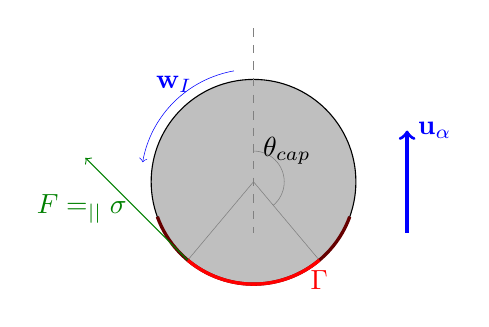
\begin{tikzpicture}[scale =1.3]
        \draw[fill=lightgray](0,0) circle (1);
        \draw[very thin,gray](230:1)--(0,0)--(310:1);
        \draw[very thin,gray](0,0)++(310:0.3) arc (-50:90:0.3)node[right,black]{$\theta_\text{cap}$};
        \draw[very thin,blue,->](0,0)++(100:1.1) arc (100:170:1.1)node[midway,above]{$\textbf{w}_I$};
        \draw[very thick,red!40!black](0,0)++(200:1) arc (200:340:1);
        \draw[very thick,red](0,0)++(230:1) arc (230:310:1)node[below]{$\Gamma$};
        \draw[very thick,blue,->](1.5,-0.5)--++(0,1)node[right]{$\textbf{u}_\alpha$};
        \draw[dashed,gray](0,1.5)--++(0,-2);
        \draw[red,->,green!50!black](230:1)--++(-1,1)node[midway,left]{$F = \nablab_{||} \sigma$};
    \end{tikzpicture}
    \caption{Schematization of the stagnant-cap regime for a
    spherical rising bubble in a quiescent liquid.}
    \label{fig:contaminated_bubbles}
\end{figure}


It can be shown that at the microscale level $C_I$ and $C_k$ follows these conservation laws \citep{pesci2018computational,manikantan2020surfactant}, 
\begin{align*}
    \pddt C_1
    + \nablabh \cdot (\textbf{u}_1 C_1)
    &= D \Delta C_1
    \;\;\; \text{on} \;\;\; \Omega_1\\
    \pddt C_I
    + \nablabhI \cdot (\textbf{u}_I C_I)
    &= D_I \Delta_{||} C_I
    \;\;\; \text{on} \;\;\; \Sigma,
\end{align*}
where $D$ and $D_I$ are the volume and surface diffusion coefficient, respectively. 
The operator $\Delta = \nablabh \cdot (\nablabh\ldots)$ and $\Delta_{||}= \nablabhI \cdot (\nablabhI\ldots)$ are the volume and surface Laplacian operator, respectively.

Now that the microscale equations are well posed we can easily derive the averaged equations for $C_1$ in the continuous phase based on \ref{eq:avg_dt_chi_f}. 
From these considerations the averaged conservation law of $C_1$ the continuous reads, 
\begin{equation}
    \pddt (\phi_1 \oneavg{C_1})
    + \nablab \cdot (\phi_1 \oneavg{C_1} \oneavg{\textbf{u}_1})
    = D \Delta (\phi_1\oneavg{C_1}) 
    - \pnavg{b_\alpha}
    +  \nablab \cdot \textbf{B}
    \label{eq:hybrid_avg_dt_C}
\end{equation}
where $b_\alpha$ is the exchange term with the dispersed phase given by, 
\begin{equation*}
    b_\alpha
    = \int_{\Sigma_\alpha}
    D(\nablabh C_1 ) 
\cdot \textbf{n}_2d\Sigma.
\end{equation*}
The interagrand of $b_\alpha$ is equivalent to the Kinetically controlled sorption boundary condition\citet{pesci2018computational}. 
We recover as in \citet{manikantan2020surfactant} that the term $D(\nablabh C_1) \cdot \textbf{n}_2$ acts as an exchange terms in the surface surfactant concentration equation. 
In \citet{manikantan2020surfactant} it is modeled as a source, denoted $j_n$ in their article.
In fact, it can b shown that Equation (3.9) of \citet{manikantan2020surfactant} correspond to \ref{eq:dt_delta_I_f_I} with $f_I = \Gamma$. 
\tb{disscus the possible closure found by \citet{kentheswaran2022direct}}
Nevertheless, due to the dispersed phase averaging process an additional term arise in the transport of the concentration $C_1$. 
Indeed, the dissipative term $B_\alpha$ can be expressed by, 
\begin{equation*}
    B_\alpha
    =     
    \frac{s_\alpha n_p}{a}\pnnavg{C_\alpha\textbf{r}_c}
    + \oneavg{C'_1\textbf{u}_1'}
    - aD\pnavg{\int_{\Sigma_\alpha} \textbf{n}_2
    (\nablabh C_1)
\cdot \textbf{n}_2d\Sigma}
\end{equation*}
The last term represent the first moment of the Kinetically controlled sorption boundary condition, together with the integrated value of $C_1$ on the surface of the particle. 


For the dispersed phase we first wish to solve an equation for the mean surface surfactant concentration $C_\alpha$. 
From \ref{eq:avg_dt_dq_alpha_tot} the averaged linear conservation equation of $C_\alpha$ reads as, 
\begin{equation}
    \pddt (\pnavg{C_\alpha})
    + \nablabh \cdot (\pnavg{\textbf{u}_\alpha} \pnnavg{C_\alpha} + \pnavg{\textbf{u}_\alpha' C'_\alpha})
    = 
    \frac{\pnavg{b_\alpha}}{s_\alpha}
    \label{eq:avg_dt_dC_alpha_tot}
\end{equation}
The fluctuation terms in \ref{eq:avg_dt_dC_alpha_tot} has great chances to be non-negligible as the rising velocity of a bubble is greatly correlated with $C_\alpha$. 
Additionally, one can notice that the diffusive term $D_I \nablabhI \Gamma$ plays no role in the resultant of surfactant. 

By making use of \ref{eq:avg_dt_dG_alpha_tot} together with \ref{eq:avg_dt_dQ_alpha_tot} we can also derive an equation for the mean position of the surfactant, $\textbf{r}_c$, along the surface. 
It has the form :
\begin{multline}
    \pddt (\pnavg{\textbf{r}_\Gamma})
    + \nablabh \cdot (\pnavg{\textbf{u}_\alpha\textbf{r}_\Gamma})
    =
    - \frac{n_p}{s_\alpha}\pnnavg{\frac{\textbf{r}_c}{C_\alpha}b_\alpha}
    + \frac{n_p}{s_\alpha}\pnnavg{
        \frac{1}{C_\alpha}
        \int_{\Sigma_\alpha} \left[
        \Gamma \textbf{w}_I
        - D_I (\nablabhI \Gamma)
    \right] d\Sigma}\\
    + \frac{n_p}{s_\alpha}\pnnavg{
    \frac{1}{C_\alpha}
    \int_{\Sigma_\alpha} \textbf{r} \left[
        D(\nablabh C_1)
    \right]\cdot \textbf{n}_2  d\Sigma}.
    \label{eq:avg_dt_dG_alpha_tot}
\end{multline}
Let examine each source terms. 
The first term on the RHS represent the change in center of surfactant due to the isotropic exchange with the bulk phase. 
The other exchange term account for the anisotropic apport of surfactant over the surface of the particle.
This term might be of great importance since the bubble's surface will absorbed more surfactant in low concentrated zone.  
The second term account for the surfactants diffusion and advection over the droplet surface. 
The latter being probably neglectable as in \citet{kentheswaran2022direct}. 
In the high area density 
In a steady state regime it be shown that $C_I \textbf{w}_I = 0$ also 



This vector directly gives a relation on the $\theta_\text{cap}$ which is correlated by the drag. 
According to the scheme
\begin{align*}
    |\textbf{r}_c| s_\alpha
    &=a^2 C_I \int_{0}^{2\pi} \int_{0}^{\theta_\text{cap}}  \sin\theta \textbf{r}_z d\phi d\theta\\
    &=a^2 C_I \int_{0}^{2\pi} \int_{0}^{\theta_\text{cap}}  \sin\theta a \cos\theta d\phi d\theta\\
    &=a^3 C_I \pi \cos^2{\theta_\text{cap}}
\end{align*}
so $r_z = \frac{1}{2}a C_I \cos^2{\theta_\text{cap}}$
Due to the complexity of the problem we won't develop further in this work. 
The main takeaway here is to understand that these first and higher order moment equation are tools to describe the dispersed phase at any order of accuracy regardless of the problem treated. 

\tb{Add "surfactant dynamic" }
\tb{with the exchange with the bulk}
\tb{Open on surfactant bubbbly flow with the JFM review and bothe}
\tb{Open non fore-after axissymmetric particle}


\tb{Extends to solid mechanics with deformable particle and composite}

\tb{
\subsubsection*{Oblate bubbles}

As it has already mentioned the trace of the moment of momentum equation can be used to derive the Reyl
It is also possible to derive from the second moment of mass equation an equation for the mean aspect ratio $\pnnavg{\xi}$ of the particles. 
Indeed, let's consider obalte particles, such as droplets or bubble, in this case the second moment of mass can be written, $\mathcal{M}_\alpha =  \textbf{pp} [M_\alpha^{||}(t) - M_\alpha^\bot(t)] +  \textbf{I} M_\alpha^\bot(t)$
\tb{As in tomiyama example they state that the shape of the particle is of particular importance here the moment of volume matter }


\subsubsection*{Spherical compressible bubbles}
As mentioned in the \ref{sec:Lagrangian} from teh trace of the moment of momentum equation we can recover the Rayleigh-Lamb-Plesset equation. 
Thus, by using the averaged moment of momentum equation we can falll back on \citet{zhang1994ensemble} model. 

\subsubsection*{Slightly deformable elastic particle}

Now let consider the momentum conservation of slightly deformable particles. 
First, the velocity field inside the particles, is assumed linear and incompressible, such that $\textbf{u}(\textbf{y}_\alpha) = \textbf{u}_\alpha + \mathcal{L}_\alpha \cdot \textbf{r}$ where the second order tensor  $\mathcal{L}_\alpha= \textbf{e}_\alpha+ \boldsymbol{\omega}$, with $\textbf{e}$ and $\boldsymbol{\omega}$ are symmetric and skew-symmetric tensors, respectively.
It directly follows from the expression of the velocity : $\mathcal{P}_\alpha = \int_{\Omega_\alpha} \textbf{r}\textbf{u} d\Omega = \mathcal{L}_\alpha\cdot \mathcal{M}$
 
The constitutive equation of the stress, $\textbf{T}_2$, within the particle phase can be written such as $\textbf{T}_2 = \mathbb{C} : \textbf{e}_2$ for elastic materials, with $\mathbb{C}$ the fourth order stiffness tensor and $ \textbf{e}_2 = \frac{1}{2}\left(\nablab\textbf{u}_2+(\nablab\textbf{u}_2)^T\right)$ is the rate of strain symmetric tensor. 
Making use of the internal velocity expression yield directly the relation, $\textbf{e}_2=\textbf{e}_\alpha\cdot$ in $\Omega_\alpha$. 

We know that the deformation of the particles will not have an explicit impact on the linear conservation equations.
Thus, we will be interested into the first and second order momentum and mass conservation equations respectively.   
Making use of the average of \ref{eq:dt_P_alpha} over every configuration of the flow, and using the previous properties yield an equation for the average stress tensor within the suspension, namely, 
\begin{equation}
    \pnnavg{\int_{\Omega_\alpha}\textbf{T}_\alpha d\Omega}
    = n_p\mathbb{C} : \pnnavg{(\mathcal{L}_\alpha+ \mathcal{L}_\alpha^T) v_\alpha}
    % = - \mathcal{L}_\alpha\cdot \mathcal{L}_\alpha\cdot \mathcal{M}_\alpha
    % - \mathcal{M}_\alpha \cdot\ddt \mathcal{L}_\alpha
    % - \textbf{M}_\alpha
    \label{eq:hybrid_avg_dt_P_alpha}
\end{equation}
\begin{equation}
    \mathcal{M}_\alpha \cdot\ddt \mathcal{L}_\alpha
    = - \mathcal{L}_\alpha\cdot \mathcal{L}_\alpha\cdot \mathcal{M}_\alpha
    - \mathbb{C} : (\mathcal{L}_\alpha+ \mathcal{L}_\alpha^T) v_\alpha
    - \textbf{M}_\alpha
    \label{eq:hybrid_avg_dt_P_alpha}
\end{equation}
Besed on that kind of argument \citet{lhuillier1987phenomenology}
}